\section{Modelagem Estrutural}
\label{sec:4.3}

A modelagem estrutural descreve a organização estática do sistema por meio das classes, seus atributos, métodos e relacionamentos. \citeonline{fowler2004} destaca que o diagrama de classes não se limita à listagem de atributos, mas expressa a estrutura estática do sistema e as relações entre suas entidades, funcionando como base para a organização do modelo.

\subsection{Diagrama de Classes}
\label{subsec:4.3.1}

O Diagrama de Classes do IGRIS apresenta a estrutura completa das entidades de domínio e seus relacionamentos. A organização reflete diretamente os módulos do backend: controle de acesso, domínio acadêmico e núcleo de otimização.

O controle de acesso é sustentado pela entidade \texttt{UsuarioPerfil}, que implementa o padrão de múltiplos perfis por usuário; um mesmo colaborador pode exercer simultaneamente as funções de professor e coordenador sem duplicação de cadastro. As entidades \texttt{Perfil}, \texttt{Link} e \texttt{TipoLink} complementam esse módulo, gerenciando permissões e o mecanismo de convite por link.

No domínio acadêmico, a classe \texttt{Curso} atua como agregadora principal, relacionando-se com \texttt{Disciplina} por meio de \texttt{DisciplinaCurso} para compor a matriz curricular, e com \texttt{Turma} para definir as ofertas semestrais. A entidade \texttt{Matriz} vincula turmas e disciplinas em um semestre específico, representando a grade curricular que alimenta o algoritmo genético. A tabela \texttt{UsuarioDisciplina} mapeia quais professores estão aptos a ministrar cada disciplina.

O núcleo do sistema é a entidade \texttt{AlocacaoGrade}, que materializa a solução do problema de timetabling ao vincular uma matriz, uma disponibilidade, uma grade e um usuário docente. Cada instância dessa entidade representa o resultado do algoritmo genético ao reunir simultaneamente a disponibilidade do professor, a necessidade da turma e a restrição de horário.

\begin{landscape}
\begin{figure}[p]
\centering
\caption{Diagrama de Classes do IGRIS}
\label{fig:diagrama_classes}
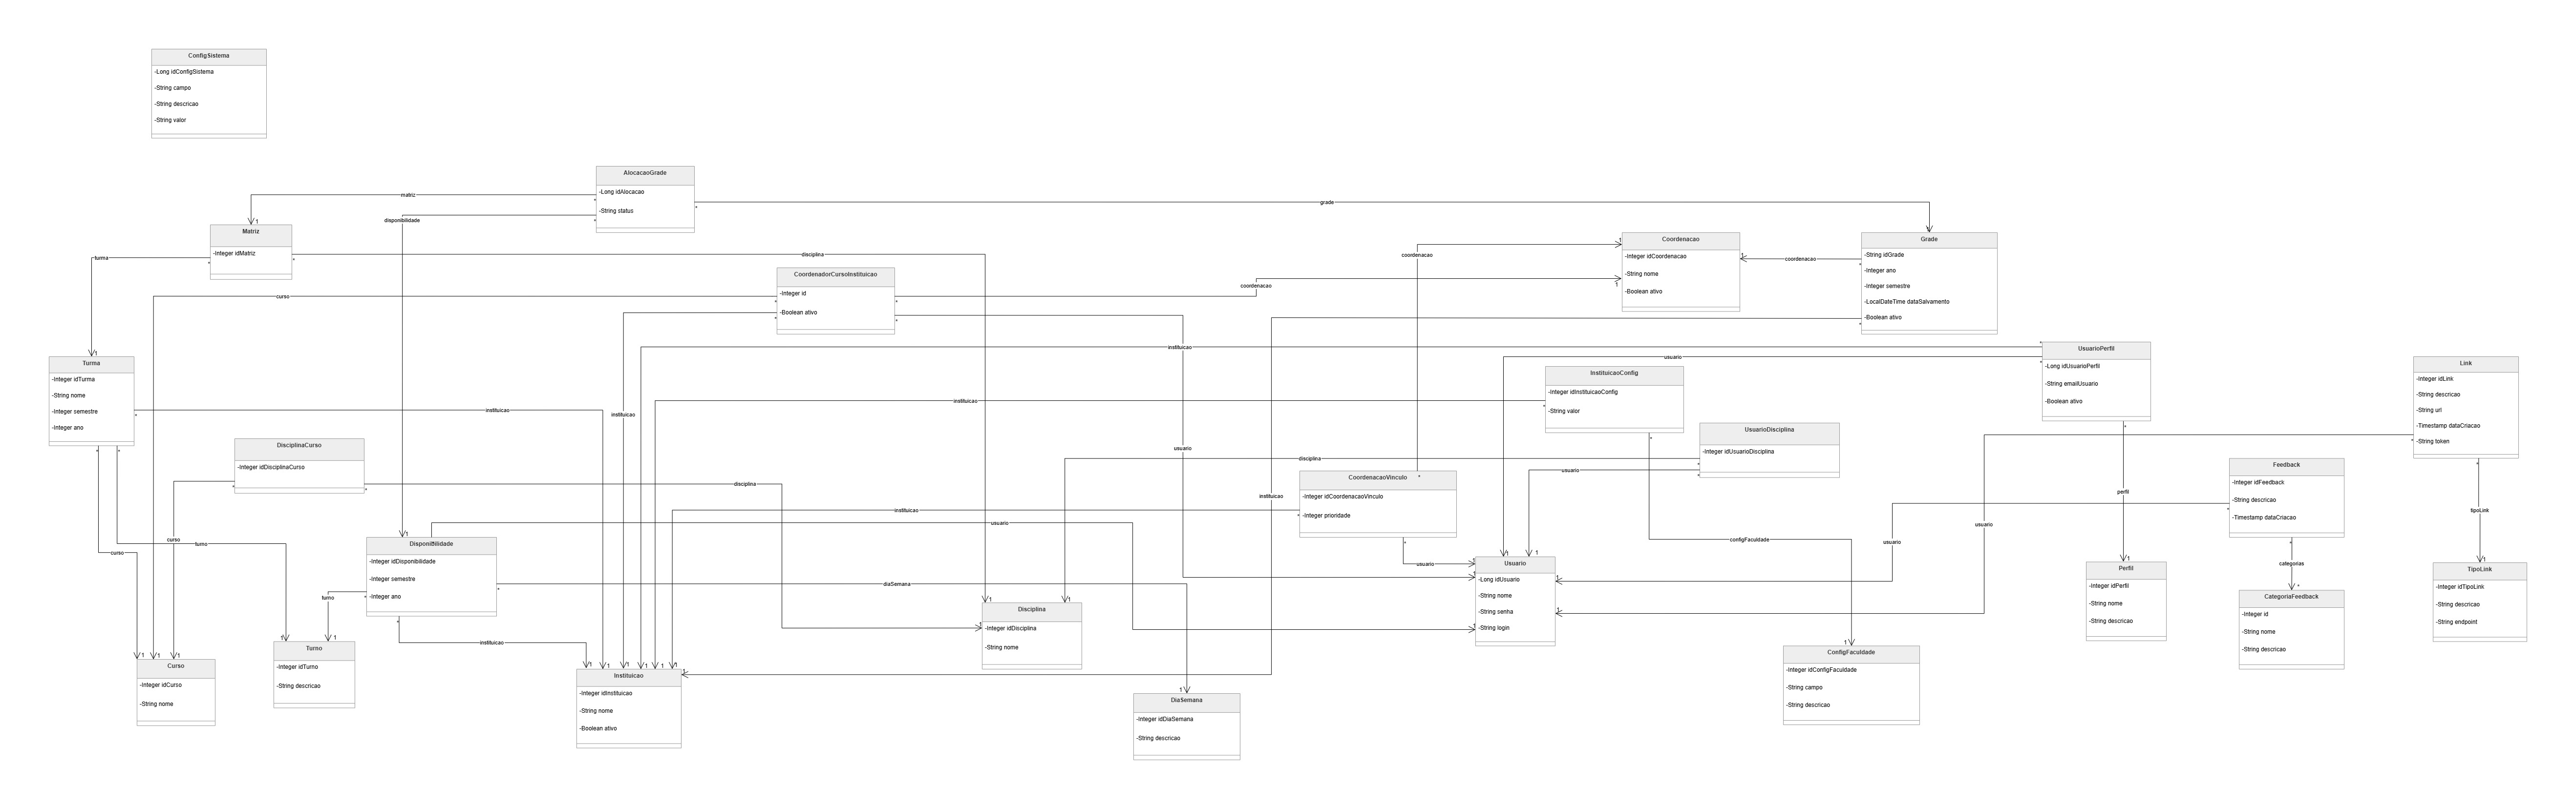
\includegraphics[width=\linewidth,height=0.9\textheight,keepaspectratio]{figuras/Figura_10_diagrama de classe.jpg}
\fonteautores
\end{figure}
\end{landscape}

\subsection{Especificação das Classes}
\label{subsec:4.3.2}

As tabelas a seguir descrevem os atributos, tipos de dados, visibilidade e semântica de cada classe identificada no modelo orientado a objetos do IGRIS, servindo como referência para a implementação das entidades de domínio.

% Tabela 64
\vspace{\baselineskip}

\Needspace{0.32\textheight}
\begin{longtable}{|L{3.5cm}|L{3.5cm}|L{3.5cm}|L{3.5cm}|}
\caption{Especificação da Classe: Instituicao} \\
\hline
\textbf{Elemento} & \textbf{Tipo/Assinatura} & \textbf{Visibilidade} & \textbf{Descrição} \\
\hline
\endfirsthead
\hline
\textbf{Elemento} & \textbf{Tipo/Assinatura} & \textbf{Visibilidade} & \textbf{Descrição} \\
\hline
\endhead
idInstituicao & int & private & Identificador único da instituição. \\
\hline
nome & String & private & Nome oficial da instituição. \\
\hline
ativo & boolean & private & Indicador se a instituição está ativa no sistema. \\
\hline
\end{longtable}

\fonteautores

% Tabela 65
\vspace{\baselineskip}

\Needspace{0.32\textheight}
\begin{longtable}{|L{3.5cm}|L{3.5cm}|L{3.5cm}|L{3.5cm}|}
\caption{Especificação da Classe: Coordenacao} \\
\hline
\textbf{Elemento} & \textbf{Tipo/Assinatura} & \textbf{Visibilidade} & \textbf{Descrição} \\
\hline
\endfirsthead
\hline
\textbf{Elemento} & \textbf{Tipo/Assinatura} & \textbf{Visibilidade} & \textbf{Descrição} \\
\hline
\endhead
idCoordenacao & int & private & Identificador da coordenação. \\
\hline
nome & String & private & Nome da coordenação (ex.: Engenharia de Software). \\
\hline
ativo & boolean & private & Indica se a coordenação está ativa. \\
\hline
instituicao & Instituicao & private & Instituição a que a coordenação pertence. \\
\hline
\end{longtable}

\fonteautores

% Tabela 66
\vspace{\baselineskip}

\Needspace{0.32\textheight}
\begin{longtable}{|L{3.5cm}|L{3.5cm}|L{3.5cm}|L{3.5cm}|}
\caption{Especificação da Classe: CoordenadorCursoInstituicao} \\
\hline
\textbf{Elemento} & \textbf{Tipo/Assinatura} & \textbf{Visibilidade} & \textbf{Descrição} \\
\hline
\endfirsthead
\hline
\textbf{Elemento} & \textbf{Tipo/Assinatura} & \textbf{Visibilidade} & \textbf{Descrição} \\
\hline
\endhead
idCoordenadorCurso & int & private & Identificador do vínculo do coordenador ao curso/instituição. \\
\hline
coordenacao & Coordenacao & private & Coordenação associada. \\
\hline
usuario & Usuario & private & Usuário que atua como coordenador. \\
\hline
instituicao & Instituicao & private & Instituição do vínculo. \\
\hline
curso & Curso & private & Curso coordenado. \\
\hline
\end{longtable}

\fonteautores

% Tabela 67
\vspace{\baselineskip}

\Needspace{0.32\textheight}
\begin{longtable}{|L{3.5cm}|L{3.5cm}|L{3.5cm}|L{3.5cm}|}
\caption{Especificação da Classe: CoordenacaoVinculo} \\
\hline
\textbf{Elemento} & \textbf{Tipo/Assinatura} & \textbf{Visibilidade} & \textbf{Descrição} \\
\hline
\endfirsthead
\hline
\textbf{Elemento} & \textbf{Tipo/Assinatura} & \textbf{Visibilidade} & \textbf{Descrição} \\
\hline
\endhead
usuario & Usuario & private & Usuário vinculado à coordenação. \\
\hline
coordenacao & Coordenacao & private & Coordenação vinculada. \\
\hline
instituicao & Instituicao & private & Instituição do vínculo. \\
\hline
prioridade & int & private & Prioridade do vínculo, usada para resolução de conflitos. \\
\hline
\end{longtable}

\fonteautores

% Tabela 68
\vspace{\baselineskip}

\Needspace{0.32\textheight}
\begin{longtable}{|L{3.5cm}|L{3.5cm}|L{3.5cm}|L{3.5cm}|}
\caption{Especificação da Classe: Curso} \\
\hline
\textbf{Elemento} & \textbf{Tipo/Assinatura} & \textbf{Visibilidade} & \textbf{Descrição} \\
\hline
\endfirsthead
\hline
\textbf{Elemento} & \textbf{Tipo/Assinatura} & \textbf{Visibilidade} & \textbf{Descrição} \\
\hline
\endhead
idCurso & int & private & Identificador do curso. \\
\hline
nome & String & private & Nome do curso (ex.: Ciência da Computação). \\
\hline
\end{longtable}

\fonteautores

% Tabela 69
\vspace{\baselineskip}

\Needspace{0.32\textheight}
\begin{longtable}{|L{3.5cm}|L{3.5cm}|L{3.5cm}|L{3.5cm}|}
\caption{Especificação da Classe: Disciplina} \\
\hline
\textbf{Elemento} & \textbf{Tipo/Assinatura} & \textbf{Visibilidade} & \textbf{Descrição} \\
\hline
\endfirsthead
\hline
\textbf{Elemento} & \textbf{Tipo/Assinatura} & \textbf{Visibilidade} & \textbf{Descrição} \\
\hline
\endhead
idDisciplina & int & private & Identificador da disciplina. \\
\hline
nome & String & private & Nome da disciplina. \\
\hline
\end{longtable}

\fonteautores

% Tabela 70
\vspace{\baselineskip}

\Needspace{0.32\textheight}
\begin{longtable}{|L{3.5cm}|L{3.5cm}|L{3.5cm}|L{3.5cm}|}
\caption{Especificação da Classe: DisciplinaCurso} \\
\hline
\textbf{Elemento} & \textbf{Tipo/Assinatura} & \textbf{Visibilidade} & \textbf{Descrição} \\
\hline
\endfirsthead
\hline
\textbf{Elemento} & \textbf{Tipo/Assinatura} & \textbf{Visibilidade} & \textbf{Descrição} \\
\hline
\endhead
idDisciplinaCurso & int & private & Identificador da associação disciplina-curso. \\
\hline
curso & Curso & private & Curso ao qual a disciplina pertence. \\
\hline
disciplina & Disciplina & private & Disciplina associada. \\
\hline
semestre & int & private & Semestre previsto na matriz curricular (quando aplicável). \\
\hline
\end{longtable}

\fonteautores

% Tabela 71
\vspace{\baselineskip}

\Needspace{0.32\textheight}
\begin{longtable}{|L{3.5cm}|L{3.5cm}|L{3.5cm}|L{3.5cm}|}
\caption{Especificação da Classe: Turma} \\
\hline
\textbf{Elemento} & \textbf{Tipo/Assinatura} & \textbf{Visibilidade} & \textbf{Descrição} \\
\hline
\endfirsthead
\hline
\textbf{Elemento} & \textbf{Tipo/Assinatura} & \textbf{Visibilidade} & \textbf{Descrição} \\
\hline
\endhead
idTurma & int & private & Identificador da turma. \\
\hline
nome & String & private & Nome/código da turma. \\
\hline
semestre & int & private & Semestre da oferta. \\
\hline
ano & int & private & Ano letivo. \\
\hline
id\_curso & int & private & Curso ao qual a turma pertence. \\
\hline
id\_turno & int & private & Turno (manhã/tarde/noite) da turma. \\
\hline
id\_instituicao & int & private & Instituição responsável. \\
\hline
\end{longtable}

\fonteautores

% Tabela 72
\vspace{\baselineskip}

\Needspace{0.32\textheight}
\begin{longtable}{|L{3.5cm}|L{3.5cm}|L{3.5cm}|L{3.5cm}|}
\caption{Especificação da Classe: Matriz} \\
\hline
\textbf{Elemento} & \textbf{Tipo/Assinatura} & \textbf{Visibilidade} & \textbf{Descrição} \\
\hline
\endfirsthead
\hline
\textbf{Elemento} & \textbf{Tipo/Assinatura} & \textbf{Visibilidade} & \textbf{Descrição} \\
\hline
\endhead
idMatriz & int & private & Identificador da matriz (grade curricular associada a uma turma/curso). \\
\hline
id\_turma & int & private & Turma relacionada à matriz. \\
\hline
id\_disciplina & int & private & Disciplina pertencente à matriz curricular. \\
\hline
semestre & int & private & Semestre em que a disciplina é prevista. \\
\hline
\end{longtable}

\fonteautores

% Tabela 73
\vspace{\baselineskip}

\Needspace{0.32\textheight}
\begin{longtable}{|L{3.5cm}|L{3.5cm}|L{3.5cm}|L{3.5cm}|}
\caption{Especificação da Classe: Usuario} \\
\hline
\textbf{Elemento} & \textbf{Tipo/Assinatura} & \textbf{Visibilidade} & \textbf{Descrição} \\
\hline
\endfirsthead
\hline
\textbf{Elemento} & \textbf{Tipo/Assinatura} & \textbf{Visibilidade} & \textbf{Descrição} \\
\hline
\endhead
idUsuario & int & private & Identificador único do usuário. \\
\hline
login & String & private & Login do usuário (único). \\
\hline
nome & String & private & Nome completo do usuário. \\
\hline
senha & String & private & Senha para autenticação (armazenada de forma segura). \\
\hline
email & String & private & E-mail de contato do usuário. \\
\hline
\end{longtable}

\fonteautores

% Tabela 74
\vspace{\baselineskip}

\Needspace{0.32\textheight}
\begin{longtable}{|L{3.5cm}|L{3.5cm}|L{3.5cm}|L{3.5cm}|}
\caption{Especificação da Classe: Perfil} \\
\hline
\textbf{Elemento} & \textbf{Tipo/Assinatura} & \textbf{Visibilidade} & \textbf{Descrição} \\
\hline
\endfirsthead
\hline
\textbf{Elemento} & \textbf{Tipo/Assinatura} & \textbf{Visibilidade} & \textbf{Descrição} \\
\hline
\endhead
idPerfil & int & private & Identificador do perfil (papel). \\
\hline
nome & String & private & Nome do perfil (ex.: Coordenador, Professor, Administrador). \\
\hline
\end{longtable}

\fonteautores

% Tabela 75
\vspace{\baselineskip}

\Needspace{0.32\textheight}
\begin{longtable}{|L{3.5cm}|L{3.5cm}|L{3.5cm}|L{3.5cm}|}
\caption{Especificação da Classe: UsuarioPerfil} \\
\hline
\textbf{Elemento} & \textbf{Tipo/Assinatura} & \textbf{Visibilidade} & \textbf{Descrição} \\
\hline
\endfirsthead
\hline
\textbf{Elemento} & \textbf{Tipo/Assinatura} & \textbf{Visibilidade} & \textbf{Descrição} \\
\hline
\endhead
idUsuarioPerfil & int & private & Identificador do vínculo entre usuário e perfil. \\
\hline
id\_usuario & int & private & Usuário associado. \\
\hline
id\_perfil & int & private & Perfil do usuário. \\
\hline
id\_instituicao & int & private & Instituição onde o perfil vale. \\
\hline
email & String & private & E-mail institucional ou contato do vínculo. \\
\hline
ativo & boolean & private & Indica se o vínculo/perfil está ativo. \\
\hline
\end{longtable}

\fonteautores

% Tabela 76
\vspace{\baselineskip}

\Needspace{0.32\textheight}
\begin{longtable}{|L{3.5cm}|L{3.5cm}|L{3.5cm}|L{3.5cm}|}
\caption{Especificação da Classe: UsuarioDisciplina} \\
\hline
\textbf{Elemento} & \textbf{Tipo/Assinatura} & \textbf{Visibilidade} & \textbf{Descrição} \\
\hline
\endfirsthead
\hline
\textbf{Elemento} & \textbf{Tipo/Assinatura} & \textbf{Visibilidade} & \textbf{Descrição} \\
\hline
\endhead
idUsuarioDisciplina & int & private & Identificador da associação usuário-disciplina. \\
\hline
id\_usuario & int & private & Professor/usuário apto a lecionar a disciplina. \\
\hline
id\_disciplina & int & private & Disciplina associada. \\
\hline
ano & int & private & Ano de referência da aptidão. \\
\hline
semestre & int & private & Semestre de referência da aptidão. \\
\hline
\end{longtable}

\fonteautores

% Tabela 77
\vspace{\baselineskip}

\Needspace{0.32\textheight}
\begin{longtable}{|L{3.5cm}|L{3.5cm}|L{3.5cm}|L{3.5cm}|}
\caption{Especificação da Classe: Disponibilidade} \\
\hline
\textbf{Elemento} & \textbf{Tipo/Assinatura} & \textbf{Visibilidade} & \textbf{Descrição} \\
\hline
\endfirsthead
\hline
\textbf{Elemento} & \textbf{Tipo/Assinatura} & \textbf{Visibilidade} & \textbf{Descrição} \\
\hline
\endhead
idDisponibilidade & int & private & Identificador da disponibilidade cadastrada. \\
\hline
semestre & int & private & Semestre a que a disponibilidade se aplica. \\
\hline
ano & int & private & Ano letivo da disponibilidade. \\
\hline
diaSemana & DiaSemana & private & Dia da semana referente. \\
\hline
usuario & Usuario & private & Usuário que registra a disponibilidade (professor). \\
\hline
turno & Turno & private & Turno disponível. \\
\hline
turma & Turma & private & Turma relacionada, quando aplicável. \\
\hline
instituicao & Instituicao & private & Instituição do registro. \\
\hline
\end{longtable}

\fonteautores

% Tabela 78
\vspace{\baselineskip}

\Needspace{0.32\textheight}
\begin{longtable}{|L{3.5cm}|L{3.5cm}|L{3.5cm}|L{3.5cm}|}
\caption{Especificação da Classe: Turno} \\
\hline
\textbf{Elemento} & \textbf{Tipo/Assinatura} & \textbf{Visibilidade} & \textbf{Descrição} \\
\hline
\endfirsthead
\hline
\textbf{Elemento} & \textbf{Tipo/Assinatura} & \textbf{Visibilidade} & \textbf{Descrição} \\
\hline
\endhead
idTurno & int & private & Identificador do turno. \\
\hline
descricao & String & private & Descrição do turno (Manhã/Tarde/Noite). \\
\hline
ativo & boolean & private & Indica se o turno está ativo no catálogo. \\
\hline
\end{longtable}

\fonteautores

% Tabela 79
\vspace{\baselineskip}

\Needspace{0.32\textheight}
\begin{longtable}{|L{3.5cm}|L{3.5cm}|L{3.5cm}|L{3.5cm}|}
\caption{Especificação da Classe: DiaSemana} \\
\hline
\textbf{Elemento} & \textbf{Tipo/Assinatura} & \textbf{Visibilidade} & \textbf{Descrição} \\
\hline
\endfirsthead
\hline
\textbf{Elemento} & \textbf{Tipo/Assinatura} & \textbf{Visibilidade} & \textbf{Descrição} \\
\hline
\endhead
idDiaSemana & int & private & Identificador do dia da semana. \\
\hline
descricao & String & private & Nome do dia (Segunda, Terça, ...). \\
\hline
ativo & boolean & private & Indica se o dia está habilitado no calendário. \\
\hline
\end{longtable}

\fonteautores

% Tabela 80
\vspace{\baselineskip}

\Needspace{0.32\textheight}
\begin{longtable}{|L{3.5cm}|L{3.5cm}|L{3.5cm}|L{3.5cm}|}
\caption{Especificação da Classe: AlocacaoGrade} \\
\hline
\textbf{Elemento} & \textbf{Tipo/Assinatura} & \textbf{Visibilidade} & \textbf{Descrição} \\
\hline
\endfirsthead
\hline
\textbf{Elemento} & \textbf{Tipo/Assinatura} & \textbf{Visibilidade} & \textbf{Descrição} \\
\hline
\endhead
idLinha & int & private & Identificador da linha de alocação na grade. \\
\hline
usuario & Usuario & private & Professor alocado. \\
\hline
disciplina & Disciplina & private & Disciplina alocada. \\
\hline
diaSemana & DiaSemana & private & Dia da semana da aula. \\
\hline
turno & Turno & private & Turno/hora da alocação. \\
\hline
turma & Turma & private & Turma alocada. \\
\hline
grade & Grade & private & Referência à grade onde a alocação pertence. \\
\hline
\end{longtable}

\fonteautores

% Tabela 81
\vspace{\baselineskip}

\Needspace{0.32\textheight}
\begin{longtable}{|L{3.5cm}|L{3.5cm}|L{3.5cm}|L{3.5cm}|}
\caption{Especificação da Classe: Grade} \\
\hline
\textbf{Elemento} & \textbf{Tipo/Assinatura} & \textbf{Visibilidade} & \textbf{Descrição} \\
\hline
\endfirsthead
\hline
\textbf{Elemento} & \textbf{Tipo/Assinatura} & \textbf{Visibilidade} & \textbf{Descrição} \\
\hline
\endhead
idGrade & String & private & Identificador da grade (pode ser GUID). \\
\hline
id\_usuario & Usuario & private & Usuário que gerou a grade (coordenador/sistema). \\
\hline
ano & int & private & Ano letivo da grade. \\
\hline
semestre & int & private & Semestre da grade. \\
\hline
dataGeracao & date & private & Timestamp da geração da grade. \\
\hline
\end{longtable}

\fonteautores

% Tabela 82
\vspace{\baselineskip}

\Needspace{0.32\textheight}
\begin{longtable}{|L{3.5cm}|L{3.5cm}|L{3.5cm}|L{3.5cm}|}
\caption{Especificação da Classe: Links} \\
\hline
\textbf{Elemento} & \textbf{Tipo/Assinatura} & \textbf{Visibilidade} & \textbf{Descrição} \\
\hline
\endfirsthead
\hline
\textbf{Elemento} & \textbf{Tipo/Assinatura} & \textbf{Visibilidade} & \textbf{Descrição} \\
\hline
\endhead
idLink & int & private & Identificador do link/recurso. \\
\hline
url & String & private & Endereço do recurso/link. \\
\hline
dtGerada & date & private & Data de geração do link/recurso. \\
\hline
horas & int & private & Tempo associado (quando aplicável). \\
\hline
tipoLink & TipoLink & private & Tipo do link (categoria). \\
\hline
usuario & Usuario & private & Usuário que criou/usa o link. \\
\hline
\end{longtable}

\fonteautores

% Tabela 83
\vspace{\baselineskip}

\Needspace{0.32\textheight}
\begin{longtable}{|L{3.5cm}|L{3.5cm}|L{3.5cm}|L{3.5cm}|}
\caption{Especificação da Classe: TipoLink} \\
\hline
\textbf{Elemento} & \textbf{Tipo/Assinatura} & \textbf{Visibilidade} & \textbf{Descrição} \\
\hline
\endfirsthead
\hline
\textbf{Elemento} & \textbf{Tipo/Assinatura} & \textbf{Visibilidade} & \textbf{Descrição} \\
\hline
\endhead
idTipoLink & int & private & Identificador do tipo de link. \\
\hline
nome & String & private & Nome do tipo de link. \\
\hline
descricao & String & private & Descrição do propósito do link. \\
\hline
\end{longtable}

\fonteautores
